% !TeX spellcheck = de_DE
\documentclass{uebung_cs}
\usepackage{algo121}
\blattname{Wochenplan: Gierige Algorithmen}

\begin{document}
\section*{Vorbereitung}
Lies E Kapitel 4 und schau das Video der Woche.

\section*{Dienstag}
\begin{aufgabe}[Dateien auf Band]
    Auf einem Magnetband sind $n$ Dateien gespeichert.
    Die Längen der Dateien sind durch ein Feld $L[1..n]$ gegeben, das heißt, die $i$-te auf dem Band gespeicherte Datei hat Länge $L[i]$.
    Um Datei $k$ zu lesen, muss das Band alle Dateien von $1$ bis $k$ lesen.
    \begin{enumerate}
        \item(\warmup) Betrachte ein Band, auf dem sechs Dateien mit $L=[8,3,1,6,4,2]$ gespeichert sind. Zum Beispiel hat Datei $1$ die Länge $8$.
        Wie hoch sind die Kosten, um Datei $4$ zu lesen?
        \item(\warmup) Wie hoch sind die erwarteten Kosten bei a), wenn ein sechsseitiger Würfel geworfen wird und die damit indizierte Datei gelesen wird?
        \item Wenn jede Datei $k$ mit Wahrscheinlichkeit $1/n$ angefragt wird, sortieren wir die Dateien am Besten der Größe nach. Jetzt aber sind manche Dateien beliebter als andere: Datei $k$ wird mit Wahrscheinlichkeit $F[k]$ angefragt. Das heißt, $F[1..n]$ ist eine Wahrscheinlichkeitsverteilung über $\{1,\dots,n\}$ und die erwarteten Kosten, um Datei~$k$ zu lesen, sind
        \[\sum_{i=1}^k F[i]\cdot L[i]\,.\]
        In welcher Reihenfolge müssen wir die Dateien jetzt sortieren, damit die erwarteten Kosten so klein wie möglich sind?
    \end{enumerate}
\end{aufgabe}

\begin{aufgabe}[Huffman-Code]\phantom{.}
    \begin{enumerate}
        \item (\warmup) Ist der folgende Code präfixfrei?
        \begin{center}
            { \ttfamily
            \begin{tabular}{c|c|c|c|c|c}
                L & R & U & D & A & B \\ \hline
                00 & 01 & 10 & 11 & 0 & 1 
            \end{tabular}
            }
        \end{center}
        \item Gegeben ist die folgende Zeichenkette $s$ über dem Alphabet:
        $$
            s = \texttt{ALGO1\textvisiblespace IST\textvisiblespace TOLL}
        $$
        \begin{enumerate}
            \item[i.] Bestimme die Häufigkeit aller Buchstaben in $s$ und erstelle den Baum des zugehörigen Huffman-Codes. Gehe dabei folgendermaßen vor:
            
            Beim Verschmelzen zweier Symbole mit minimaler Häufigkeit wird das resultierende Symbol durch eine lexikographisch geordnete Liste der Buchstaben beider Symbole dargestellt. Stehen mehrere Symbole mit minimaler Häufigkeit zur Auswahl, wähle diejenigen aus, welche unter der lexikographischen Ordnung am kleinsten sind. Hierbei ist für die einzelnen Buchstaben die folgende Ordnung vorgegeben:
            \begin{center}
                {\ttfamily \textvisiblespace\ $\leq$ 1 $\leq$ A $\leq$ G $\leq$ I $\leq$ L $\leq$ O $\leq$ S $\leq$ T}.
            \end{center}
            \item[ii.] Erstelle noch einen Huffman-Code, diesmal unter Verwendung der folgenden Ordnung:
            \begin{center}
                {\ttfamily \textvisiblespace\ $\leq$ T $\leq$ O $\leq$ A $\leq$ S $\leq$ L $\leq$ G $\leq$ I $\leq$ 1}.
            \end{center}
        \end{enumerate}
        \item Codiere die folgende Zeichenkette unter Verwendung des Huffman-Codes aus Teilaufgabe b) i.:
        \begin{center}
            \ttfamily 1\textvisiblespace TOAST\textvisiblespace TATTOO
        \end{center}
    \end{enumerate}
\end{aufgabe}

\begin{aufgabe}[Per Hand laufen lassen]\phantom{.}
    \begin{enumerate}
        \item Verwende den gierigen Algorithmus aus der Vorlesung, um auf der folgenden Eingabe einen maximalen konfliktfreien Stundenplan $\{s_{i_1}, s_{i_2}, \dots, s_{i_k}\}$ zu bestimmen:
        \begin{center}
            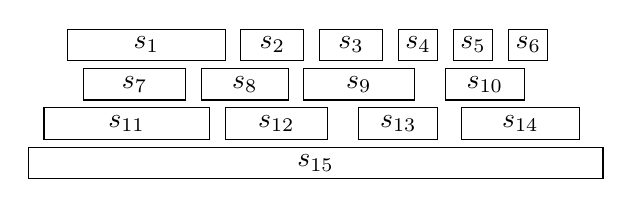
\begin{tikzpicture}
                \draw (0,4) rectangle node{$s_1$} (2,3.6);
                \draw (2.2,4) rectangle node{$s_2$} (3,3.6);
                \draw (3.2,4) rectangle node{$s_3$} (4,3.6);
                \draw (4.2,4) rectangle node{$s_4$} (4.7,3.6);
                \draw (4.9,4) rectangle node{$s_5$} (5.4,3.6);
                \draw (5.6,4) rectangle node{$s_6$} (6.1,3.6);

                \draw (0.2,3.5) rectangle node{$s_7$} (1.5,3.1);
                \draw (1.7,3.5) rectangle node{$s_8$} (2.8,3.1);
                \draw (3,3.5) rectangle node{$s_9$} (4.4,3.1);
                \draw (4.8,3.5) rectangle node{$s_{10}$} (5.8,3.1);

                \draw (-0.3,3) rectangle node{$s_{11}$} (1.8,2.6);
                \draw (2,3) rectangle node{$s_{12}$} (3.3,2.6);
                \draw (3.7,3) rectangle node{$s_{13}$} (4.7,2.6);
                \draw (5,3) rectangle node{$s_{14}$} (6.5,2.6);

                \draw (-0.5,2.5) rectangle node{$s_{15}$} (6.8,2.1);
            \end{tikzpicture}
        \end{center}
        \item Verwende den gierigen Algorithmus aus der Vorlesung, um auf dem folgenden Graphen ein stabiles Matching zu bestimmen:
    \end{enumerate}
\end{aufgabe}

\begin{aufgabe}[Andere Scheduling-Strategie]\phantom{.}
    \begin{enumerate}
        \item Verwende folgende gierige Strategie, um auf der folgenden Eingabe einen Stundenplan zu berechnen:
        \begin{itemize}
            \item[-] Sortiere die Vorlesungen absteigend nach dem Zeitpunkt ihres Endes
            \item[-] Belege die nächste konfliktfreie Vorlesung
            \item[-] Wiederhole 
        \end{itemize}
        \item Finde eine Eingabe, auf der die Strategie aus der vorigen Teilaufgabe einen Stundenplan berechnet, welcher \textbf{nicht} maximal ist.
    \end{enumerate}
\end{aufgabe}

\begin{aufgabe}[Scheduling]
    Gegeben sind Startzeiten $S[1..n]$ und Endzeiten $F[1..n]$ von $n$ Vorlesungen.
    \begin{enumerate}
        \item(\warmup) Beschreibe mathematisch (also durch eine logische Formel, die $S$ und $F$ benutzt), was es heißt, dass die Zeiten von Vorlesung $i$ und $j$ sich überlappen.
        \item Professorin S. Chedule hat folgende Idee, um den gierigen Algorithmus für das Scheduling zu vereinfachen: Anstatt nach den Endzeiten, sortieren wir die Vorlesung nach den Startzeiten, und nehmen also immer die erste Vorlesung in den Stundenplan auf, die als nächstes startet und keinen Konflikt verursacht. Finde ein Gegenbeispiel, in dem dieser Algorithmus fehlschlägt.
    \end{enumerate}
\end{aufgabe}


\begin{aufgabe}[Huffman-Codierung]
    Betrachte das Alphabet $\{\texttt a,\ \texttt l,\ \texttt g,\ \texttt o,\ \texttt t,\ \texttt i,\ \texttt s\}$ mit der folgenden Häufigkeitstabelle:
	\begin{center}
		\begin{tabular}{ccccccc}
			\texttt{a}&\texttt{l}&\texttt{g}&\texttt{o}&\texttt{t}&\texttt{i}&\texttt{s}\\\hline
			3&3&1&1&7&2&4\\
		\end{tabular}
	\end{center}
    \begin{enumerate}
        \item Führe den Algorithmus zur Huffman-Codierung für diese Häufigkeitstabelle aus und gib jeden Zwischenschritt an.
        \item Gib einen optimalen binären Code an. Gib für jedes Zeichen das zugehörige Codewort an, und male den zugehörigen Binärbaum.
    \end{enumerate}
\end{aufgabe}


\section*{Donnerstag}
\begin{aufgabe}[Maximum Cut]

\end{aufgabe}

\begin{aufgabe}[Balance]
    
\end{aufgabe}
    
\begin{aufgabe}[Stabiles Matching]
\end{aufgabe}

\end{document}
